%!TEX root = ../thesis.tex

\chapter{Background}
\label{ch:background}

This thesis marries open problems in population genetics with powerful mathematical tools.
As few readers will likely have substantial exposure to both fields, we devote this initial chapter to providing preliminaries.

\section{Population Genetics}

Mathematical population genetics is concerned with X

\section{Biology}

In this section we present background.
This section is intended to motivate the problems discussed.
More specific background relevant to the applications described in Part \ref{part:application_microorganism} and Part \ref{part:applications_human} is presented in those Parts.

\subsection{Phylogenetics}

Phylogenetics is how you build a tree from evolutionary characters.

Start with sequences.
Perform an alignment.
From an alignment, one can then directly use parsimony or likelihood approaches.
Alternatively, one can compute a matrix of pairwise distances and then construct a tree that best approximates these distances.
Most relevant to this thesis are the distance-based approaches (because they can be viewed as finite metric spaces amenable to topological analysis).
Only in the case of perfectly additive data will a tree be able to exactly fit the matrix.
Identifying the pairwise distance matrix with a its finite metric space representation allows most of the results described here.

Include discussion of rooted vs unrooted.

\subsection{Distance Matrix Methods}

Introduced by Cavalli-Sforza and Edwards in 1967 \cite{CavalliSforza:1967th} and Fitch and Margoliash in 1967 \cite{Fitch:1967we}.
Compute a matrix of pairwise distances and then find the tree that best approximates those distances.
Weighted and unweighted least squares.
UPGMA.
Neighbor joining is now the most common distance-matrix approach because it can perfectly reconstruct an additive tree.
Neighbor joining was introduced by Saitou and Nei in 1987 \cite{Saitou:1987wo}.

There are limitations of distance based methods.
Do not use all the information.

Need to include discussion of metrics on aligned sequences.

\subsection{The Coalescent}

The coalescent process is a stochastic model that generates the genealogy of individuals sampled from an evolving population \cite{Wakeley:2009}.
The genealogy is then used to simulate the genetic sequences of the sample.
This model is essential to many methods commonly used in population genetics.
Starting with a present-day sample of $n$ individuals, each individual's lineage is traced backward in time, towards a mutual common ancestor.
Two separate lineages collapse via a coalescence event, representing the sharing of an ancestor by the two lineages.
The stochastic process ends when all lineages of all sampled individuals collapse into a single common ancestor.
In this process, if the total (diploid) population size $N$ is sufficiently large, then the expected time before a coalescence event, in units of $2N$ generations, is approximately exponentially distributed:
\begin{equation}
P(T_{k}=t) \approx \binom{k}{2} e ^{-\binom{k}{2} t},
\end{equation}
where $T_k$ is the time that it takes for $k$ individual lineages to collapse into $k-1$ lineages.

After generating a genealogy, the genetic sequences of the sample can be simulated by placing mutations on the individual branches of the lineage.
The number of mutations on each branch is Poisson-distributed with mean $\theta t / 2$, where $t$ is the branch length and $\theta$ is the population-scaled mutation rate.
In this model, the average \emph{genetic distance} between any two sampled individuals, defined by the number of mutations separating them, is $\theta$.

The coalescent with recombination is an extension of this model that allows different genetic loci to have different genealogies.
Looking backward in time, recombination is modeled as a splitting event, occurring at a rate determined by population-scaled recombination rate $\rho$, such that an individual has a different ancestor at different loci.
Evolutionary histories are no longer represented by a tree, but rather by an \emph{ancestral recombination graph}.
Recombination is the component of the model generating nontrivial topology by introducing deviations from a contractibile tree structure, and is the component which we would like to quantify.
Coalescent simulations were performed using \texttt{ms} \cite{Hudson:2002}.

% \begin{figure}
% \begin{center}
% \centerline{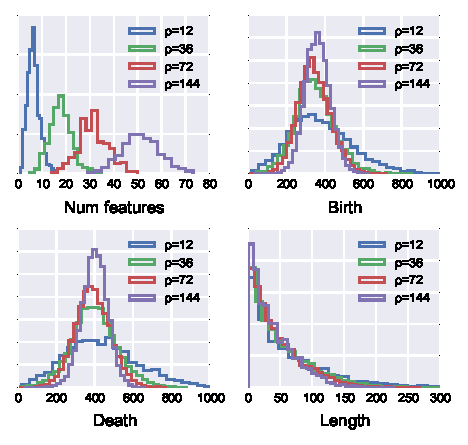
\includegraphics[width=\columnwidth]{./fig/coalescent_sims.pdf}}
% \caption{Distributions of statistics defined on the $H_1$ persistence diagram for different model parameters. Top left: Number of features. Top right: Birth time distribution. Bottom left: Death time distribution. Bottom right: Feature length distribution. Data generated from $1000$ coalescent simulations with $n=100$, $\theta=500$, and variable $\rho$.}
% \label{fig:coalescent_sims}
% \end{center}
% \end{figure}

\subsection{Horizontal Gene Transfer}

Here we should include discussion of nonvertical evolutionary processes.
This will include references to Doolittle, Koonin, Gogarten.
Lateral Gene Transfer.
Species Trees and Gene Trees.
Recombination and reassortment.
We will want to include discussion of 

\section{Algebraic Topology}

Algebriac topology associates algebraic structures to qualitative notions of shape.
Principle tool is group theory.
Groups count connected components.

\subsection{Simplicial Complexes}

Abstract Simplicial Complex
Cech Complex.
Rips Complex.

\section{Topological Data Analysis}

For excellent review of topological data analysis, see the reviews.

\subsection{Mapper}

Can compare to dimensionality reduction.
But is basically clustering.

\subsection{Persistent Homology}
\label{subsec:persistent_homology}

We summarize persistent homology from the perspective of an end-user.
For detailed background, see the reviews \cite{Carlsson:2009a,Ghrist:2008} and the books \cite{Edelsbrunner:2010,Zomorodian:2005b}.
In brief, persistent homology computes topological invariants representing information about the connectivity and holes in a dataset.
A dataset, $S=(s_{1},\ldots,s_{N})$, is represented as a point cloud in a high-dimensional space (not necessarily Euclidean).
From the point cloud, a nested family of simplicial complexes, or a filtration, is constructed, parameterized by a filtration value $\epsilon$, which controls the simplices present in the complex.
The two most common ways of constructing a simplicial complex at each $\epsilon$ are the \Cech complex and the Vietoris-Rips complex.
The filtration is represented as a list of simplices defined on the vertices of $S$, annotated with the $\epsilon$ at which the simplex appears.
Given a filtration, the persistence algorithm is used to compute homology groups.
The $0$-dimensional homology ($H_0$) represents a hierarchical clustering of the data.
Higher dimensional homology groups represent loops, holes, and higher dimensional voids in the data.
Each feature is annotated with an interval, representing the $\epsilon$ at which the feature appears and the $\epsilon$ at which the feature contracts in the filtration.
These filtration values are the \emph{birth} and \emph{death} times, respectively.
The topological invariants in the filtration can be concisely represented in a barcode diagram, a set of line segments ordered by filtration value on the horizontal axis (Figure XXX).
Equivalently, invariants can represented by a persistence diagram, a scatter plot with the birth time on the horizontal axis and the death time on the vertical axis.

Several packages for computing persistent homology have been developed [Dionysus, Javaplex, Guidi] and TDA frontend for R.
Persistent homology is computed using Dionysus \cite{Morozov:2012}.

\subsection{Statistical Persistent Homology}

Cutting edge in TDA.
Primarily motivated by the idea that there is a true topology and we are given a finite sample of it.
We are motivated by a slightly different problem in this thesis.
We briefly discuss these results.
Persistence Landscapes.


\subsection{Multidimensional Persistence}

